\documentclass[a4paper]{article}
\usepackage[T1]{fontenc}			% \chapter package
\usepackage[english]{babel}
\usepackage[english]{isodate}  		% date format
\usepackage{graphicx}				% manage images
\usepackage{subcaption}             % manage subfigures
\usepackage{amsfonts}
\usepackage{booktabs}				% high quality tables
\usepackage{amsmath}				% math package
\usepackage{amssymb}				% another math package (e.g. \nexists)
\usepackage{bm}                     % bold math symbols
\usepackage{mathtools}				% emphasize equations
\usepackage{amsthm}					% better theorems
\usepackage{enumitem}				% manage list
\usepackage{pifont}					% nice itemize
\usepackage{cancel}					% cancel math equations
\usepackage{caption}				% custom caption
\usepackage[]{mdframed}				% box text
\usepackage{multirow}				% more lines in a table
\usepackage[x11names]{xcolor}		% RGB color
\usepackage[many]{tcolorbox}		% colorful box
\usepackage{listings}
\usepackage{qrcode}
\usepackage{fontawesome5}
\usepackage{ragged2e}
\usepackage{cite}                   % references
\usepackage{imakeidx}               % index
\makeindex[program=makeindex, columns=1,
           title=Index, 
           intoc,
           options={-s index-style.ist}]
\usepackage{fancyhdr}

%\pdfcompresslevel=0
%\pdfobjcompresslevel=0

\definecolor{codegreen}{rgb}{0,0.6,0}
\definecolor{codegray}{rgb}{0.5,0.5,0.5}
\definecolor{codepurple}{rgb}{0.58,0,0.82}
\definecolor{backcolour}{rgb}{255,255,255}
\lstdefinestyle{mystyle}{
    backgroundcolor=\color{backcolour},   
	commentstyle=\color{codegreen},
	keywordstyle=\color{magenta},
	numberstyle=\tiny\color{codegray},
	stringstyle=\color{codepurple},
	basicstyle=\ttfamily\footnotesize,
	breakatwhitespace=false,         
	breaklines=true,                 
	captionpos=b,                    
	keepspaces=true,                 
	numbers=left,                    
	numbersep=5pt,                  
	showspaces=false,                
	showstringspaces=false,
	showtabs=false,                  
	tabsize=2,
    mathescape,
    frame=lines
}
\lstset{style=mystyle}


% thanks Mico: https://tex.stackexchange.com/a/60218/312896
\makeatletter
\renewcommand\paragraph{\@startsection{paragraph}{4}{\z@}%
            {-2.5ex\@plus -1ex \@minus -.25ex}%
            {1.25ex \@plus .25ex}%
            {\normalfont\normalsize\bfseries}}
\makeatother
\setcounter{secnumdepth}{4} % how many sectioning levels to assign numbers to
\setcounter{tocdepth}{4}    % how many sectioning levels to show in ToC


% draw a frame around given text
\newcommand{\framedtext}[1]{%
	\par%
	\noindent\fbox{%
		\parbox{\dimexpr\linewidth-2\fboxsep-2\fboxrule}{#1}%
	}%
}


% table of content links
\usepackage{xcolor}
\usepackage[linkcolor=black, citecolor=blue, urlcolor=cyan]{hyperref} % hypertexnames=false
\hypersetup{
	colorlinks=true
}


\newtheorem{theorem}{\textcolor{Red3}{\underline{Theorem}}}
\newtheorem{lemma}[theorem]{\textcolor{Red3}{\underline{Lemma}}}
\renewcommand{\qedsymbol}{QED}
\newcommand{\dquotes}[1]{``#1''}
\newcommand{\longline}{\noindent\rule{\textwidth}{0.4pt}}
\newcommand{\circledtext}[1]{\raisebox{.5pt}{\textcircled{\raisebox{-.9pt}{#1}}}}
\newcommand{\definition}[1]{\textcolor{Red3}{\textbf{#1}}\index{#1}}
\newcommand{\blackdefinition}[1]{\textbf{#1}\index{#1}}
\newcommand{\definitionWithSpecificIndex}[3]{\textcolor{Red3}{\textbf{#1}}\index{#2}\index{#3}}
\newcommand{\example}[1]{\textcolor{Green4}{\textbf{#1}}}
\newcommand{\highspace}{\vspace{1.2em}\noindent}
\renewcommand{\lstlistingname}{Algorithm}
\renewcommand{\lstlistlistingname}{Algorithms}
\newcommand{\version}{v0.4.0-dev}


\begin{document}
    \newcounter{definition}[section]
    \newcounter{example}[section]
    \newcounter{exercise}[section]
    
    \newtcolorbox[use counter = definition]{definitionbox}[1][]{%
        breakable,
        enhanced,
        colback=red!5!white,
        colframe=red!75!black,
        fonttitle=\bfseries,
        title={Definition \thetcbcounter#1} %
    }

    \newtcolorbox[use counter = exercise]{exercisebox}[1][]{%
        breakable,
        enhanced,
        colback=Red3!5!white,
        colframe=Red3!75!black,
        fonttitle=\bfseries,
        title={Exercise \thetcbcounter#1} %
    }
    
    \newtcolorbox[use counter = example]{examplebox}[1][]{%
        breakable,
        enhanced,
        colback=Green4!5!white,
        colframe=Green4!75!black,
        fonttitle=\bfseries,
        title={Example \thetcbcounter#1} %
    }

    \newtcolorbox[]{deepeningbox}[1][]{%
        breakable,
        enhanced,
        colback=DarkOrange3!5!white,
        colframe=DarkOrange3!75!black,
        fonttitle=\bfseries,
        title={Deepening#1} %
    }

    %%%%%%%%%%%%%%%
    % Notes cover %
    %%%%%%%%%%%%%%%
    \author{260236}
\title{Parallel Computing - Notes - \version}
\date{\printdayoff\today}
\maketitle

    %%%%%%%%%%%
    % Preface %
    %%%%%%%%%%%
	\section*{Preface}

Every theory section in these notes has been taken from the sources:
\begin{itemize}
    \item Course slides.\cite{numerical-linear-algebra-polimi}
\end{itemize}
About:
\begin{itemize}
    \item[\faIcon{github}] \href{https://github.com/PoliMI-HPC-E-notes-projects-AndreVale69/HPC-E-PoliMI-university-notes}{GitHub repository}
    \begin{center}
        \qrcode{https://github.com/PoliMI-HPC-E-notes-projects-AndreVale69/HPC-E-PoliMI-university-notes}
    \end{center}
\end{itemize}
These notes are an unofficial resource and shouldn't replace the course material or any other book on numerical linear algebra. It is not made for commercial purposes. I've made the following notes to help me improve my knowledge and maybe it can be helpful for everyone.

As I have highlighted, a student should choose the teacher's material or a book on the topic. These notes can only be a helpful material.

\highspace

\subsection*{Correlated Projects}

During the Numerical Linear Algebra for HPC course, I was part of a team where we created a project that included two challenges related to the course. See more details in the corresponding repository:
\begin{itemize}
    \item[\faIcon{github}] \href{https://github.com/PoliMI-HPC-E-notes-projects-AndreVale69/NLA-challenges}{GitHub repository}
    \begin{center}
        \qrcode{https://github.com/PoliMI-HPC-E-notes-projects-AndreVale69/NLA-challenges}
    \end{center}
\end{itemize}

    %%%%%%%%%%%%%%%%%%%%%
    % Table of contents %
    %%%%%%%%%%%%%%%%%%%%%
    \tableofcontents
    \newpage

    %%%%%%%%%%%%%%%%%%%
    % Fancy pagestyle %
    %%%%%%%%%%%%%%%%%%%
    \pagestyle{fancy}
    \fancyhead{} % clear all header fields
    \fancyhead[R]{\nouppercase{\leftmark\hfill\rightmark}}

    %%%%%%%%
    % PRAM %
    %%%%%%%%
    \section{PRAM}

\subsection{Prerequisites}

Before we introduce the PRAM model, we need to cover some useful topics.
\begin{itemize}
    \item A \definition{Machine Model} describes a \dquotes{machine}. It gives a value to the operations on the machine. It is necessary because: it makes it easy to deal with algorithms; it achieves complexity bounds; it analyses maximum parallelism.

    \item A \definition{Random Access Machine (RAM)} is a model of computation that describes an abstract machine in the general class of register machines. Some features are:
    \begin{itemize}
        \item \textbf{Unbounded} number of local memory cells;
        \item Each memory cell can hold an integer of \textbf{unbounded} size;
        \item Instruction set includes simple operations, data operations, comparator, branches;
        \item All operations take \textbf{unit time};
        \item The definition of \textbf{time complexity} is the number of instructions executed;
        \item The definition of \textbf{space complexity} is the number of memory cells used.
    \end{itemize}
\end{itemize} % and definition
    \subsection{How it works}

\subsubsection{Computation}

A single \textbf{processor} of the PRAM, at each computation, is \textbf{composed of 5 phases} (carried out in parallel by all the processors):
\begin{enumerate}
    \item \textbf{Reads a value from one of the cells} $X\left(1\right), \dots, X\left(N\right)$
    \item Reads one of the shared memory cells $A\left(1\right), A\left(2\right), \dots$
    \item Performs some internal computation
    \item \textbf{May write into one of the output cells} $Y\left(1\right), Y\left(2\right), \dots$
    \item May write into one of the shared memory cells $A\left(1\right), A\left(2\right), \dots$
\end{enumerate}

\longline

\subsubsection{PRAM Classificiation}

During execution, a subset of processors may remain idle. Also, some processors can read from the same cell at the same time (not really a problem), but they could also try to write to the same cell at the same time (\textbf{write conflict}). For these reasons, PRAMs are classified according to their read/write capabilities (realistic and useful):
\begin{itemize}
    \item \definition{Exclusive Read (ER)}. All processors can simultaneously read from distinct memory locations.
    
    \item \definition{Exclusive Write (EW)}. All processors can simultaneously write to distinct memory locations.
    
    \item \definition{Concurrent Read (CR)}. All processors can simultaneously read from any memory location.

    \item \definition{Concurrent Write (CW)}. All processors can write to any memory location.
    \begin{flushleft}
        \textcolor{Green3}{\faIcon{question-circle} \textbf{But what value is ultimately written?}}
    \end{flushleft}
    It depends on the mode we choose:
    \begin{itemize}
        \item \definition{Priority Concurrent Write}. Processors have priority based on which value is decided, the \textbf{highest priority is allowed to complete write}.

        \item \definition{Common Concurrent Write}. All processors are allowed to complete write \textbf{if and only if all the value to be written are equal}.
        
        Any \textbf{algorithm} for this model has to \textbf{make sure that this condition is satisfied}. \textbf{Otherwise}, the \textbf{algorithm is illegal} and the \textbf{machine state will be undefined}.

        \item \definitionWithSpecificIndex{Arbitrary/Random Concurrent Write}{Arbitrary Concurrent Write}{Random Concurrent Write}. One \textbf{randomly} chosen \textbf{processor is allowed to complete write}.
    \end{itemize}
\end{itemize}

\subsubsection{Strengths of PRAM}

PRAM is attractive and important model for designers of parallel algorithms because:
\begin{itemize}
    \item It is \textbf{natural}. The number of operations executed per one cycle on $P$ processors is at most $P$ (equal to $P$ is the ideal case).

    \item It is \textbf{strong}. Any processor can read/write any shared memory cell in unit time.

    \item It is \textbf{simple}. It abstracts from any communication or synchronization overhead, which makes the complexity and correctness of PRAM algorithm easier.

    \item It can be used as a \textbf{benchmark}. If a problem has no feasible/efficient solution on PRAM, it has no feasible/efficient solution for any parallel machine.
\end{itemize}

\longline

\subsubsection{How to compare PRAM models}

Consider two generic PRAMs, models $A$ and $B$. Model $A$ is \textbf{computationally stronger} than model $B$ ($A \ge B$) \textbf{if and only if} \textbf{any algorithm} written for model $B$ will \textbf{run unchanged} on model $A$ in the \textbf{same parallel time} and with the \textbf{same basic properties}.

\highspace
However, there are some useful metrics that can be used to compare models:
\begin{itemize}
    \item \textbf{Time to solve problem} of \textbf{input size} $n$ on \textbf{\underline{one} processor}, using \textbf{best \underline{sequential} algorithm}:
    \begin{equation}
        T^{*}\left(n\right)
    \end{equation}

    \item \textbf{Time} to solve problem of input size $n$ on \underline{$\mathbf{p}$} \textbf{processors}:
    \begin{equation}
        T_{p}\left(n\right)
    \end{equation}

    \item \textbf{Speedup on $\mathbf{p}$ processors}:
    \begin{equation}
        \mathrm{SU}_{p}\left(n\right) = \dfrac{T^{*}\left(n\right)}{T_{p}\left(n\right)}
    \end{equation}

    \item \textbf{Efficiency}, which is the work done by a processor to solve a problem of input size $n$ divided by the work done by $p$ processors:
    \begin{equation}
        E_{p}\left(n\right) = \dfrac{T_{1}\left(n\right)}{pT_{p}\left(n\right)}
    \end{equation}

    \item \textbf{Shortest run time} on any process $p$:
    \begin{equation}
        T_{\infty}\left(n\right)
    \end{equation}

    \item \textbf{Cost}, equal to processors and time:
    \begin{equation}
        C\left(n\right) = P\left(n\right) \cdot T\left(n\right)
    \end{equation}

    \item \textbf{Work}, equal to the total \textbf{number of operations}:
    \begin{equation}
        W\left(n\right)
    \end{equation}
\end{itemize}
Some properties on the metrics:
\begin{itemize}
    \item The time to solve a problem of input $n$ on a single processor using the best sequential algorithm \emph{is not equal to} the time to solve a problem of input $n$ in parallel using one of the $p$ processors available. In other words, \textbf{the problem should not be solvable on a single processor on a parallel machine} (otherwise, what would be the point of using a parallel model?)
    \begin{equation*}
        T^{*} \ne T_{1}
    \end{equation*}

    \item $\mathrm{SU}_{P} \le P$

    \item $\mathrm{SU}_{P} \le \dfrac{T_{1}}{T_{\infty}}$

    \item $E_{p} \le 1$

    \item $T_{1} \ge T^{*} \ge T_{p} \ge T_{\infty}$

    \item $T^{*} \approx T_{1} \Rightarrow E_{p} \approx \dfrac{T^{*}}{pT_{p}} = \dfrac{\mathrm{SU}_{p}}{p}$

    \item $E_{p} = \dfrac{T_{1}}{pT_{p}} \le \dfrac{T_{1}}{pT_{\infty}}$

    \item $T_{1} \in O\left(C\right),  T_{p} \in O\left(\dfrac{C}{p}\right)$

    \item $W \le C$

    \item $p \approx \text{AREA} \hspace{1em} W \approx \text{ENERGY} \hspace{1em} \dfrac{W}{T_{p}} \approx \text{POWER}$
\end{itemize}
    \subsection{MVM algorithm}

The \definition{Matrix-Vector Multiply (MVM) algorithm} consists of four steps:
\begin{enumerate}
    \item \textbf{Concurrent read of vector} $X\left(1 : n\right)$ (transfer $N$ elements);

    \item \textbf{Simultaneous reads of different sections of the general matrix} $A$ (transfer $\dfrac{n^{2}}{p}$ elements to each processor);

    \item \textbf{Compute} $\dfrac{n^{2}}{p}$ operations per processor;

    \item \textbf{Simultaneous writes} (transfer $\dfrac{n}{p}$ elements from each processor).
\end{enumerate}
Let $i$ be the processor index, so the MVM algorithm is simply written as:
\begin{lstlisting}[mathescape=true, caption={Matrix-Vector Multiply (MVM)}]
GLOBAL READ (Z $\leftarrow$ X)
GLOBAL READ (B $\leftarrow A_{i}$)
COMPUTE (W := BZ)
GLOBAL WRITE (W $\rightarrow y _{i}$)
\end{lstlisting}

\highspace
\begin{figure}[!htp]
    \centering
    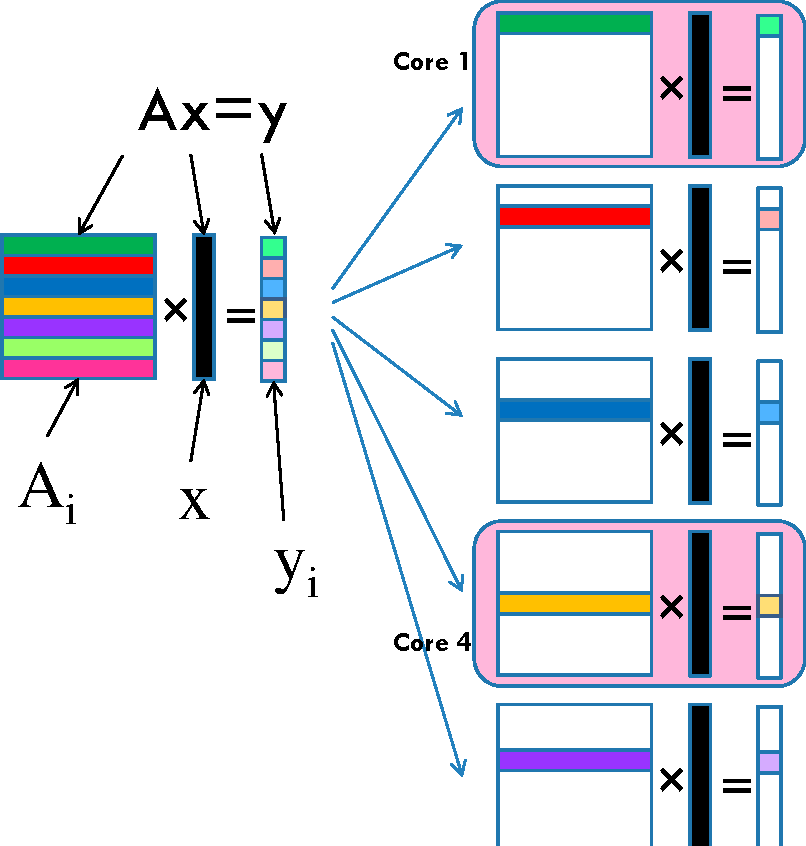
\includegraphics[width=.7\textwidth]{img/mvm-1.pdf}
    \caption{Example of MVM algorithm.}
\end{figure}

\newpage

\noindent
The performance of the MVM algorithm is as follows:
\begin{itemize}
    \item The \textbf{time to solve} a problem of size $n^{2}$ is equal to the big $O$ of the squared size of the problem as input divided by the number of processors available:
    \begin{equation*}
        T_{p}\left(n^{2}\right) = O\left(\dfrac{n^{2}}{p}\right)
    \end{equation*}
    
    \item The \textbf{cost} is equal to the number of processors and the time it takes to solve the problem. So it is quite trivial:
    \begin{equation*}
        C = O\left(\cancel{P} \cdot \dfrac{n^{2}}{\cancel{p}}\right) = O\left(n^{2}\right)
    \end{equation*}

    \item The \textbf{work} is equal to the cost, and the \textbf{linear power} $P$ is equal to the ratio of work and time to solve the problem on $p$ processors:
    \begin{equation*}
        W = C \hspace{2em} \dfrac{W}{T_{p}} = P
    \end{equation*}

    \item The \textbf{perfect efficiency} is equal to:
    \begin{equation*}
        E_{p} = \dfrac{T_{1}}{pT_{p}} = \dfrac{n^{2}}{p\frac{n^{2}}{p}} = 1
    \end{equation*}
\end{itemize}
    \subsection{SPMD sum}

The \definition{Single Program Multiple Data (SPMD)} is a term that has been used to \textbf{describe computational models} for exploiting parallelism, where \textbf{multiple processors work together to execute a program to get results faster}.

\highspace
In this section, we will see an SPMD approach on a Parallel Random Access Machine (PRAM). We will introduce one of the most common and simple mathematical operations: the sum.

\highspace
The following pseudocode takes as \textbf{input an array} of size $n = 2^{k}$. In this case, $n$ is a power of 2 because it ensures that the array can be evenly divided at each step of the computation. The value $k$ is the number of iterations or levels of the summation process.
\begin{lstlisting}[mathescape=true, caption={Single Program Multiple Data (SPMD) sum}]
BEGIN
    GLOBAL READ (A $\leftarrow$ A(I))
    GLOBAL WRITE (A $\rightarrow$ B(I))
    FOR H = 1 : K
        IF $i \le n \div 2^{h}$ THEN BEGIN
            GLOBAL READ (X $\leftarrow$ B(2$i$ - 1))
            GLOBAL READ (Y $\leftarrow$ B(2$i$))
            Z := X + Y
            GLOBAL WRITE (Z $\rightarrow$ B($i$))
        END
    IF I = 1 THEN
        GLOBAL WRITE (Z $\rightarrow$ S)
END
\end{lstlisting}
\begin{itemize}
    \item First, read the entire input array \texttt{A} and copy the read data to another array \texttt{B}.
    
    \item Loop over \texttt{h} (\texttt{1 to k}). In each iteration, for each index $i$ less than or equal to $n \div 2^{h}$, read values from array \texttt{B} at positions $2i-1$ and $2i$; sum these values (and store the result in \texttt{Z}) and store the result (\texttt{Z}) back into \texttt{B($i$)}.
    
    \item Once all iterations are complete, the final sum is stored in a variable \texttt{S}.
\end{itemize}
For example, if $n = 8$, then $k$ would be 3, meaning that the algorithm will run for 3 iterations to sum all the elements in parallel.
\begin{table}[!htp]
    \centering
    \begin{tabular}{@{} c c c @{}}
        \toprule
        $h$ & $i$ & adding \\
        \midrule
        \multirow{4}{*}{1} & 1 & 1,2 \\
          & 2 & 3,4 \\
          & 3 & 5,6 \\
          & 4 & 7,8 \\
        \cmidrule{1-3}
        \multirow{2}{*}{2} & 1 & 1,2 \\
          & 2 & 3,4 \\
        \cmidrule{1-3}
        3 & 1 & 1,2 \\
        \bottomrule
    \end{tabular}
\end{table}

\newpage

\begin{figure}[!htp]
    \centering
    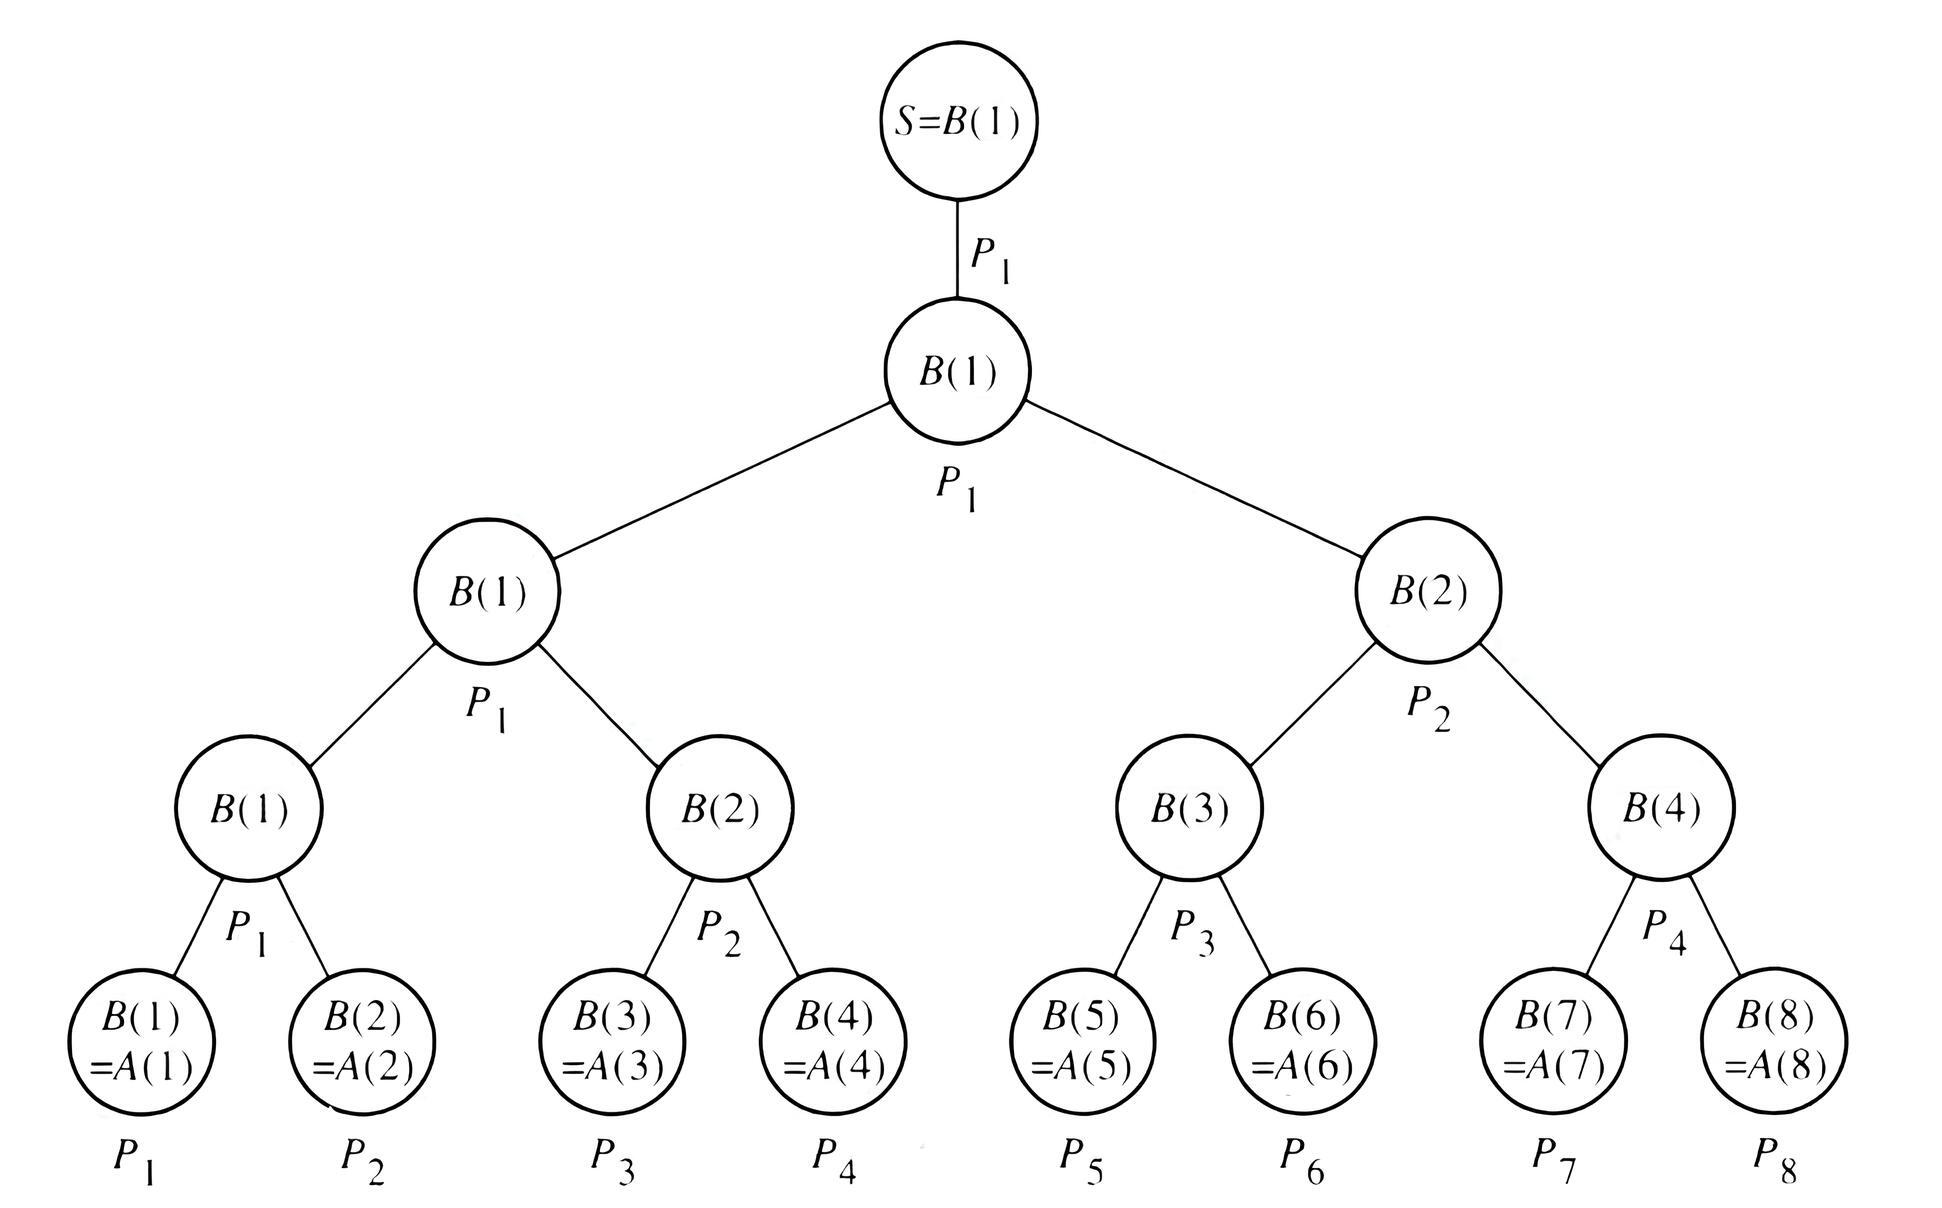
\includegraphics[width=\textwidth]{img/SPDM-sum-1.jpg}
    \caption{Computation of the sum of eight elements on a PRAM with eight processors. Each internal node represents a sum operation. The specific processor executing the operation is indicated below each node.}
    \label{fig: SPDM-sum-1}
\end{figure}

\begin{flushleft}
    \textcolor{Green3}{\faIcon{tachometer-alt} \textbf{Performance of sum}}
\end{flushleft}
When the size of the array is equal to the number of processors ($N = P$), the \textbf{speedup and efficiency decrease}:
\begin{itemize}
    \item $T^{*}\left(N\right) = T_{1}\left(N\right) = N$
    \item $T_{N=P}\left(N\right) = 2 + \log N$
    \item $\mathrm{SU}_{P} = \dfrac{N}{2+\log N}$
    \item $T^{*}\left(N\right) = P \cdot \left(2 + \log N\right) \approx N \log N$
    \item $E_{p} = \dfrac{T_{1}}{pT_{p}} = \dfrac{N}{N \log N} = \dfrac{1}{\log N}$
\end{itemize}
\begin{figure}[!htp]
    \centering
    \begin{subfigure}[h]{0.45\linewidth}
        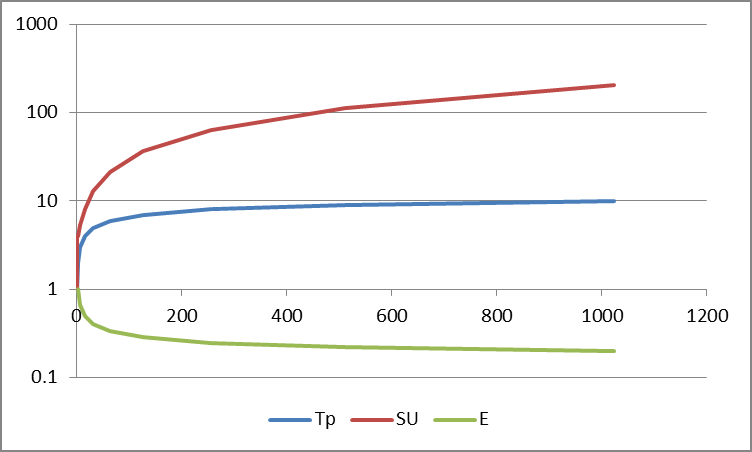
\includegraphics[width=\linewidth]{img/SPDM-sum-2.png}
    \end{subfigure}
    \hfill
    \begin{subfigure}[h]{0.45\linewidth}
        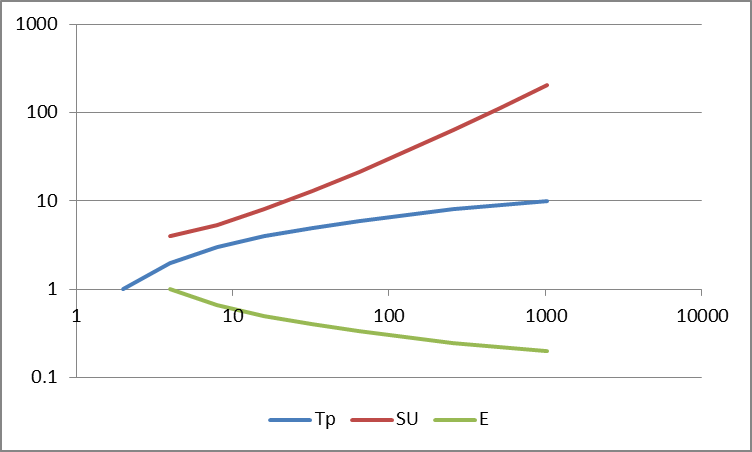
\includegraphics[width=\linewidth]{img/SPDM-sum-3.png}
    \end{subfigure}
\end{figure}

\newpage

\noindent
If the size of the array is much larger than the number of processors ($N \gg P$), the \textbf{speedup and power are linear}, the \textbf{cost is fixed} and the \textbf{efficiency is maximum (equal to 1)}:
\begin{itemize}
    \item $T^{*}\left(N\right) = T_{1}\left(N\right) = N$
    \item $T_{p}\left(N\right) = \dfrac{N}{p} + \log p$
    \item $\mathrm{SU}_{P} = \dfrac{N}{\frac{N}{p}+\log p} \approx P$
    \item $\text{COST} = p\left(\dfrac{N}{p} + \log p\right) \approx N$
    \item $\text{WORK} = N + P \approx N$
    \item $E_{p} = \dfrac{T_{1}}{pT_{p}} = \dfrac{N}{p\left(\frac{N}{p} + \log p\right)} \approx 1$
\end{itemize}
\begin{figure}[!htp]
    \centering
    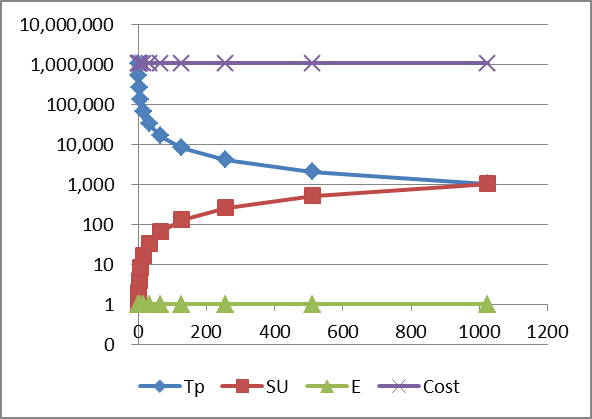
\includegraphics[width=.5\linewidth]{img/SPDM-sum-4.png}
    \caption*{$n = 1'000'000$}
\end{figure}

\begin{examplebox}
    Refer to Figure \ref{fig: SPDM-sum-1} (page \pageref{fig: SPDM-sum-1}), the performance metrics are:
    \begin{itemize}
        \item $T_{8} = 5$
        \item $C = 8 \cdot 5 = 40$ (could do 40 steps)
        \item $W = 2n = 16$ (16 on 40, wasted 24)
        \item $E_{p} = \dfrac{2}{\log n} = \dfrac{2}{3} = 0.67$
        \item $\dfrac{W}{C} = \dfrac{16}{40} = 0.4$
    \end{itemize}
\end{examplebox}
    \subsection{MM algorithm}

The \definition{Matrix Multiply (MM) algorithm} consists of three steps:
\begin{enumerate}
    \item \textbf{Compute the two matrices} $A_{i,l}$ and $B_{l,j}$, so use the concurrent read.
    \item Make the \textbf{sum}.
    \item \textbf{Store} the result using exclusive write.
\end{enumerate}
\begin{lstlisting}[mathescape=true, caption={Matrix Multiply (MM)}]
BEGIN
    $T_{i,j,l}$ = $A_{i,l} B_{l,j}$
    FOR = H = 1 : K
        IF $l \le n \div 2^{h}$ THEN
            $T_{i,j,l}$ = $T_{i,j,2l-1}$ + $T_{i,j,2l}$
    IF $l = 1$ THEN
        $C_{i,j}$ = $T_{i,j,1}$
END
\end{lstlisting}
\begin{flushleft}
    \textcolor{Green3}{\faIcon{tachometer-alt} \textbf{Performance of MM}}
\end{flushleft}
\begin{itemize}
    \item $T_{1} = n^{3}$
    \item $T_{p = n^{3}} = \log n$
    \item $\mathrm{SU} = \dfrac{n^{3}}{\log n}$
    \item $\text{Cost} = n^{3} \log n$
    \item $E_{p} = \dfrac{T_{1}}{pT_{p}} = \dfrac{1}{\log n}$
\end{itemize}
\begin{figure}[!htp]
    \centering
    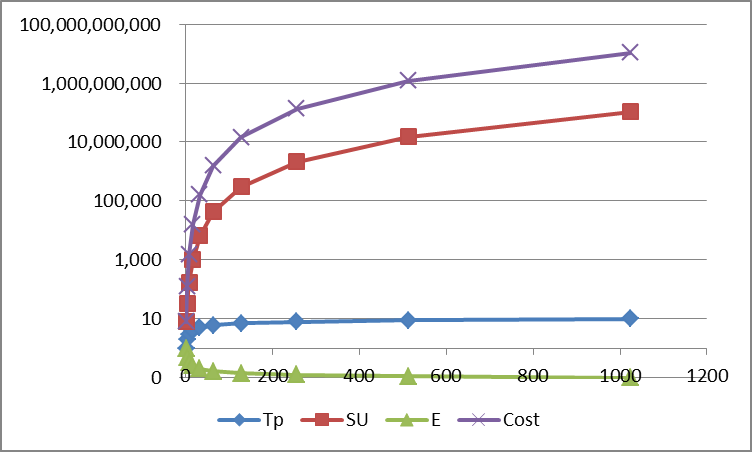
\includegraphics[width=.6\textwidth]{img/mm-1.png}
\end{figure}
    \subsection{PRAM variants and Lemmas}

The PRAM model presented here is one of the most commonly used. However, there are other important variants:
\begin{itemize}
    \item PRAM model with a \textbf{limited number of shared memory cells} (small memory PRAM). If the input data set exceeds the capacity of the shared memory, the I/O values can be evenly distributed among the processors.
    
    \item PRAM model with \textbf{limited number of processors} (small PRAM). If the number of execution threads is higher, processors can interleave multiple threads.

    \item PRAM model with \textbf{limited size of one machine word}.
    
    \item PRAM model with \textbf{access conflicts handling}. These are restrictions on simultaneous access to shared memory cells.
\end{itemize}

\begin{lemma}
    Assume $P' < P$ and same size of shared memory. Any problem that can be solved for a $P$ processor PRAM in $T$ steps can be solved in a $P'$ processor PRAM in:
    \begin{equation}
        T' = O\left(\dfrac{TP}{P'}\right)
    \end{equation}
\end{lemma}
\begin{proof}
    Partition $P$ is simulated processors into $P'$ groups of size $\frac{P}{P'}$ each. Associate each of the $P'$ simulating processors with one of these groups. Each of the simulating processors simulates one step of its group of processors by:
    \begin{itemize}
        \item Executing all their read and local computation substeps first;
        \item Executing their write substeps then.
    \end{itemize}
\end{proof}

\highspace
\begin{lemma}
    Assume $M' < M$. Any problem that can be solved for a $P$ processor and $M$-cell PRAM in $T$ steps can be solved on a $\max\left(P, M'\right)$-processors $M'$-cell PRAM in $O\left(\dfrac{TM}{M'}\right)$ steps.
\end{lemma}
\begin{proof}
    Partition $M$ simulated shared memory cells into $M'$ continuous segments $S$, of size $\frac{M}{M'}$ each. Each simulating processor $P_{I}'$ ($1 \le I \le P$), will simulate processor $P_{I}$ of the original PRAM. Each simulating processor $P_{I}'$ ($1 \le I \le M'$), stores the initial contents of $S_{I}$ into its local memory and will use $M'\left[I\right]$ as an auxiliary memory cell for simulation of accesses to cell of $S_{I}$.

    \noindent
    Simulation of one original read operation:
    \begin{lstlisting}[mathescape=true]
EACH $P_{I}'$ $\left(I = 1, \dots, \max\left(P, M'\right)\right)$ REPEATS FOR K = 1, ..., $\frac{M}{M'}$
    WRITE THE VALUE OF THE K-TH CELL OF $S_{I}$ INTO $M'\left[I\right]$ $\left(I = 1, \dots, M'\right)$
    READ THE VALUE WHICH THE SIMULATED PROCESSOR $P_{I}$ $\left(I = 1, \dots, P\right)$ WOULD READ IN THIS SIMULATED SUBSTEP, IF IT APPEARED IN THE SHARED MEMORY\end{lstlisting}
    The local computation substep of $P_{I}$ ($I = 1, \dots, P$) is simulated in one step by $P_{I}'$. SImulation of one original write operation is analogous to that of read.
\end{proof}

    \subsection{PRAM implementation}

The PRAM is an ideal model for creating parallel algorithms. Now we look at \dquotes{\emph{is it really implementable?}} The short answer is yes.

\highspace
The longest answer is the following. There are already some examples of PRAM being converted to real machine models, such as \href{https://en.wikipedia.org/wiki/Explicit_multi-threading}{Explicit Multi-Threading \break (XMT)}, Rigel, Tilera, etc. If conversion is not easy or possible, the implementation can be \dquotes{\emph{direct}}:
\begin{itemize}
    \item The concurrent read is implemented as a detect-and-multicast technique.
    \item The concurrent write is implemented depending on the end result we want to achieve. Fetch-and-operate and prefix-sum are examples of serialized writing; otherwise, the CRCW technique is used:
    \begin{itemize}
        \item Common CRCW: detect and merge
        \item Priority CRCW: detect-and-priorities
        \item Arbitrary CRCW: arbitrary
    \end{itemize}
\end{itemize}

\begin{examplebox}[: Boolean DNF (sum of products) common CRCW]
    A logical formula is considered to be in DNF if it is a disjunction of one or more conjunctions of one or more literals.

    Consider $X$ as the sum of products of AND/OR operations:
    \begin{equation*}
        X = a_{1}b_{1} + a_{2}b_{2} + \dots
    \end{equation*}
    The PRAM code, with $X$ initialized to $0$ and task index equal to \$, is:
    \begin{center}
        \texttt{if ($a_{\$}b_{\$}$) X = 1;}
    \end{center}
    The common result is that not all processors write $X$ and those that do write 1. The time complexity is $O\left(1\right)$. It works on common, priority and arbitrary CRCW.
\end{examplebox}

\noindent
Despite the previous example, exists also the PRAM SoP for the concurrent write. Let boolean $X$ as:
\begin{equation*}
    X = a_{1}b_{1} + a_{2}b_{2} + \dots
\end{equation*}
The PRAM algorithm is:
\begin{center}
    \texttt{if ($a_{i}b_{i}$) X = 1;}
\end{center}
Where all cores which write into $X$, \textbf{write the same value}.

\newpage

\begin{flushleft}
    \textcolor{Green3}{\faIcon{check} \textbf{PRAM advantages}}
\end{flushleft}
\begin{itemize}
    \item Large body of algorithms.
    \item Easy to think about it.
    \item Sync version of shared memory. It eliminates sync and common issues, allows focus on algorithms, but allows adding these issues and allows conversion to async versions.
    \item Exists architectures for both synch (PRAM) and async (SM) model.
    \item PRAM algorithms can be mapped to other models.
\end{itemize}
    \subsection{Amdahl's and Gustafson's Laws}

The \definition{Amdahl's Law} is a formula which gives the \textbf{theoretical speedup in latency of the execution of a task at fixed workload that can be expected of a system whose resources are improved}. The law can be stated as:
\begin{definitionbox}[: Amdahl's Law]
    \textbf{The overall performance improvement gained by optimizing a single part of a system is limited by the fraction of time that the improved part is actually used.}
\end{definitionbox}

\noindent
In practice, Amdahl's law says that the computation consists of interleaved segments of two types:
\begin{enumerate}
    \item \textbf{Serial segments} (which cannot be parallelized);
    \item \textbf{Parallelizable segments}.
\end{enumerate}
Therefore, the metrics we can obtain are the time on $P$ processors metric, that it is greater than the fraction of time on a processor divided by the processors $P$, and the speedup metric, that it is less than the number of processors $P$:
\begin{equation*}
    T_{P} > \dfrac{T_{1}}{P} \hspace{2em} SU < P
\end{equation*}
Graphically, we can see a fixed part of the line, which is the \textbf{serial segment} (no speedup), and a set of instructions that can be \textbf{parallelized} (the sum of these segments is equal to the unit time $1$).
\begin{figure}[!htp]
    \centering
    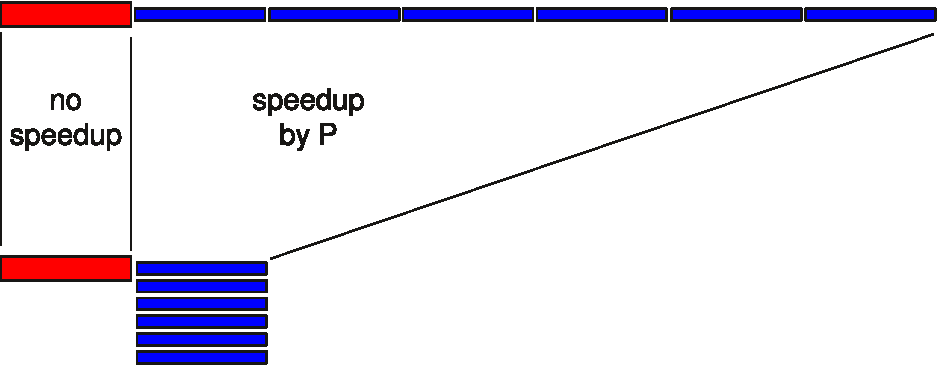
\includegraphics[width=\textwidth]{img/amdahl-law-1.pdf}
\end{figure}

\noindent
Furthermore, if we identify the parallelizable segment as $f$ and the serial segment as $1-f$, we obtain the following expressions:
\begin{equation}
    \begin{array}{rcl}
        SU\left(P,f\right) &=& \dfrac{T_{1}}{T_{P}} = \dfrac{T_{1}}{T_{1} \cdot \left(1-f\right) + \frac{T_{1}\cdot f}{P}} = \dfrac{1}{\left(1-f\right) + \frac{f}{P}} \\ [1em]
        \lim\limits_{P \rightarrow \infty}SU\left(P,f\right) &=& \dfrac{1}{1-f}
    \end{array}
\end{equation}

\highspace
In the following figure we can see the speedup with parameter $f$. Note the pessimism: for a problem with inherent $f=90\%$, there is no point in using more than 10 processors.
\begin{figure}[!htp]
    \centering
    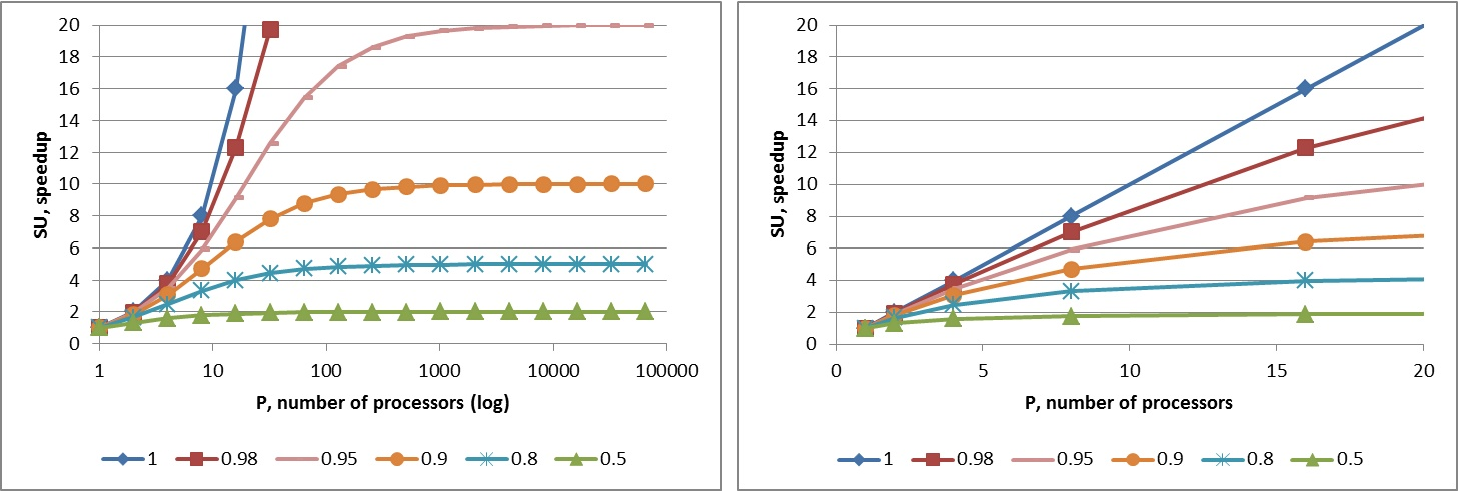
\includegraphics[width=\textwidth]{img/amdahl-law-2.pdf}
    \caption{Amdahl's law, $SU\left(P\right)$, parameter $f$.}
\end{figure}

\noindent
The original paper presenting Amdahl's Law\cite{amdahl2007validity} can be viewed by clicking on the link below or by scanning the QR code.
\begin{center}
    \href{https://ieeexplore.ieee.org/abstract/document/4785615}{Amdahl's Law}
    \hspace{2em}
    \qrcode{https://ieeexplore.ieee.org/abstract/document/4785615}
\end{center}
\textbf{Amdahl's law applies only to the cases where the problem size is fixed}. In practice, as more computing resources become available, they tend to get used on larger problems (larger datasets), and the time spent in the parallelizable part often grows much faster than the inherently serial work. In this case, \textbf{Gustafson's law gives a less pessimistic and more realistic assessment of the parallel performance}.\cite{mccool2012structured}

\highspace
\definition{Gustafson's Law} gives the speedup in the execution time of a task that theoretically gains from parallel computing, using a hypothetical run of the task on a single-core machine as the baseline. To put it another way, it is the \textbf{theoretical \dquotes{slowdown} of an already parallelized task if running on a serial machine}.

\highspace
Against Amdahl's law, Gustafson suggests the following ideas:
\begin{itemize}
    \item Portion $f$ is not fixed;
    \item The absolute serial time is fixed;
    \item Parallel problem size is increased to exploit more processors;
    \item Fixed serial time ($s$ of total) and fixed parallel time ($1-s$ of total) are invariants;
    \item \textbf{Fixed time model} and not fixed size model (as Amdahl's law):
    \begin{equation}
        SU\left(P\right) = \dfrac{T_{1}}{T_{P}} = \dfrac{s+P\cdot\left(1-s\right)}{s+\left(1-s\right)} = s + P\cdot\left(1-s\right)
    \end{equation}
\end{itemize}

\newpage

\noindent
Gustafson's law suggests a \textbf{linear speedup} and is \textbf{empirically applicable to highly parallel algorithms}.
\begin{figure}[!htp]
    \centering
    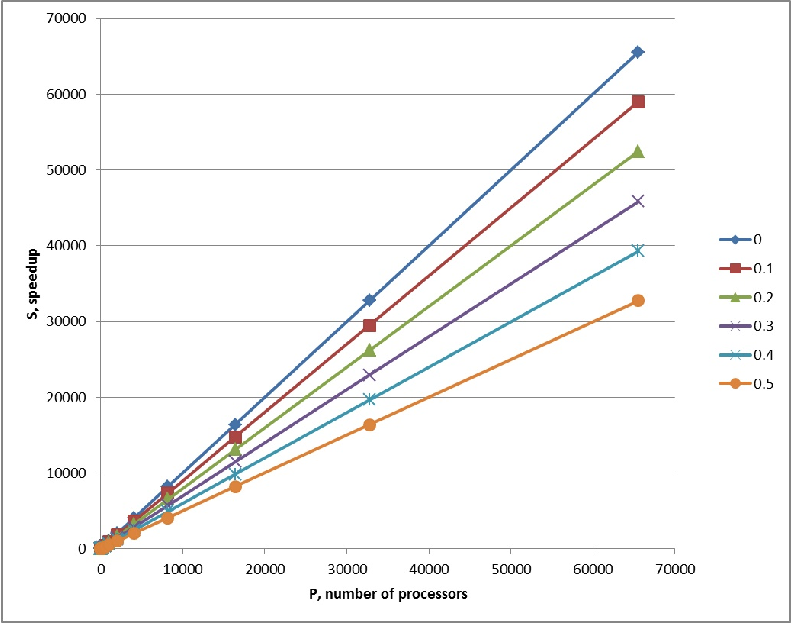
\includegraphics[width=.7\textwidth]{img/gustafson-law-1.pdf}
    \caption{Gustafson's law.}
\end{figure}

\noindent
\textbf{\emph{Amdahl's Law}} states that as computing power increases, computational requirements remain the same. In other words, the \textbf{analysis of the same data will take less time with more computing power}.

\textbf{\emph{Gustafson}}, on the other hand, argues that \textbf{more computing power leads to more careful and complete analysis of the data}. Where it would not have been possible or practical to simulate the impact of nuclear denotation on every building, car, and their contents (including furniture, structural strength, etc.) because such a calculation would have taken more time than was available to provide an answer, the increase in computing power will prompt researchers to add more data to more fully simulate more variables, giving a more accurate result.

\highspace
The original paper presenting Gustafson's Law\cite{gustafson1988reevaluating} can be viewed by clicking on the link below or by scanning the QR code.
\begin{center}
    \href{https://dl.acm.org/doi/abs/10.1145/42411.42415}{Gustafson's Law}
    \hspace{2em}
    \qrcode{https://dl.acm.org/doi/abs/10.1145/42411.42415}
\end{center}

    %%%%%%%%%%%%%%%%%%%%%%%%%%%%%%%%
    % Fundamentals of architecture %
    %%%%%%%%%%%%%%%%%%%%%%%%%%%%%%%%
    \section{Fundamentals of architecture}

\subsection{Introduction}

\subsubsection{Simplest processor}

Inside a computer, a processor executes instructions.
\begin{itemize}
    \item \textbf{Fetch/Decode}: Determine which instruction to run next;
    \item \textbf{ALU} (execution unit): Performs the operation described by an instruction, which may change values in the processor's registers or the computer's memory;
    \item \textbf{Registers}: maintain program state, store values of variables used as inputs and outputs to operations.
\end{itemize}
The simplest and most basic processor executes \textbf{one instruction per clock cycle}.
\begin{figure}[!htp]
    \centering
    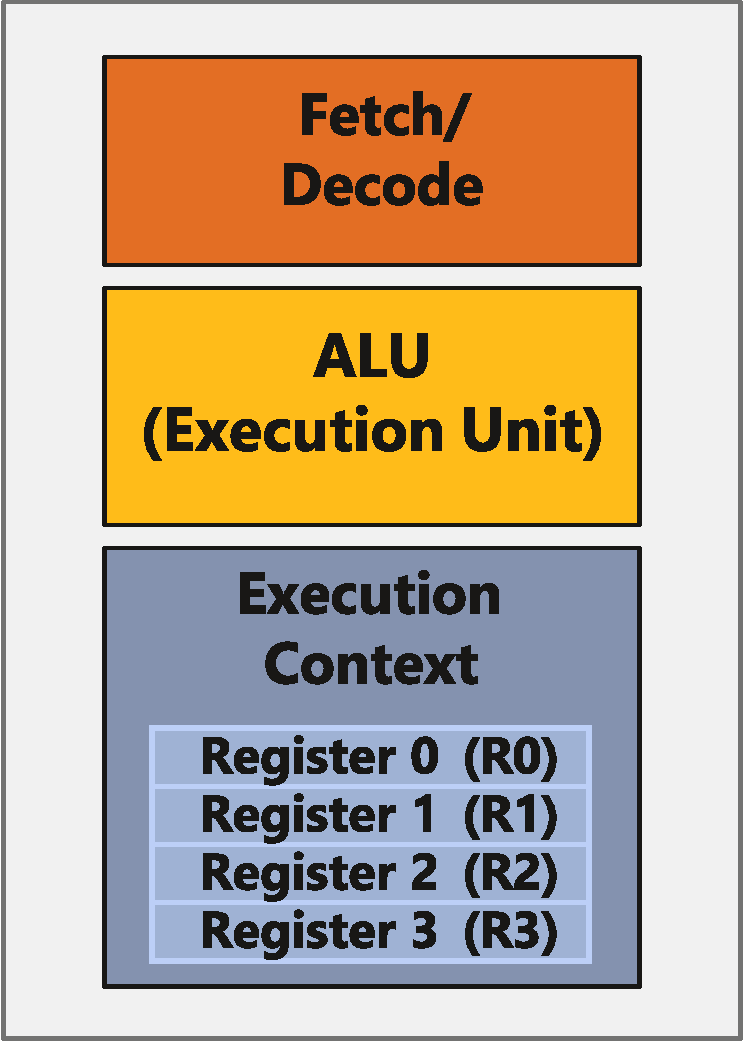
\includegraphics[width=.3\textwidth]{img/simplest-prcoessor-1.pdf}
    \caption{The simplest and most basic processor.}
\end{figure}

\newpage

\subsubsection{Superscalar processor}
A more \dquotes{complex} and realistic model is the \definitionWithSpecificIndex{superscalar processor}{Superscalar Processor}. This \textbf{processor can decode and execute up to \underline{two instructions per clock}}. The execution is slightly different from the simplest processor. The \textbf{processor automatically finds independent instructions in an instruction sequence and can execute them in parallel on multiple execution units}.
\begin{figure}[!htp]
    \centering
    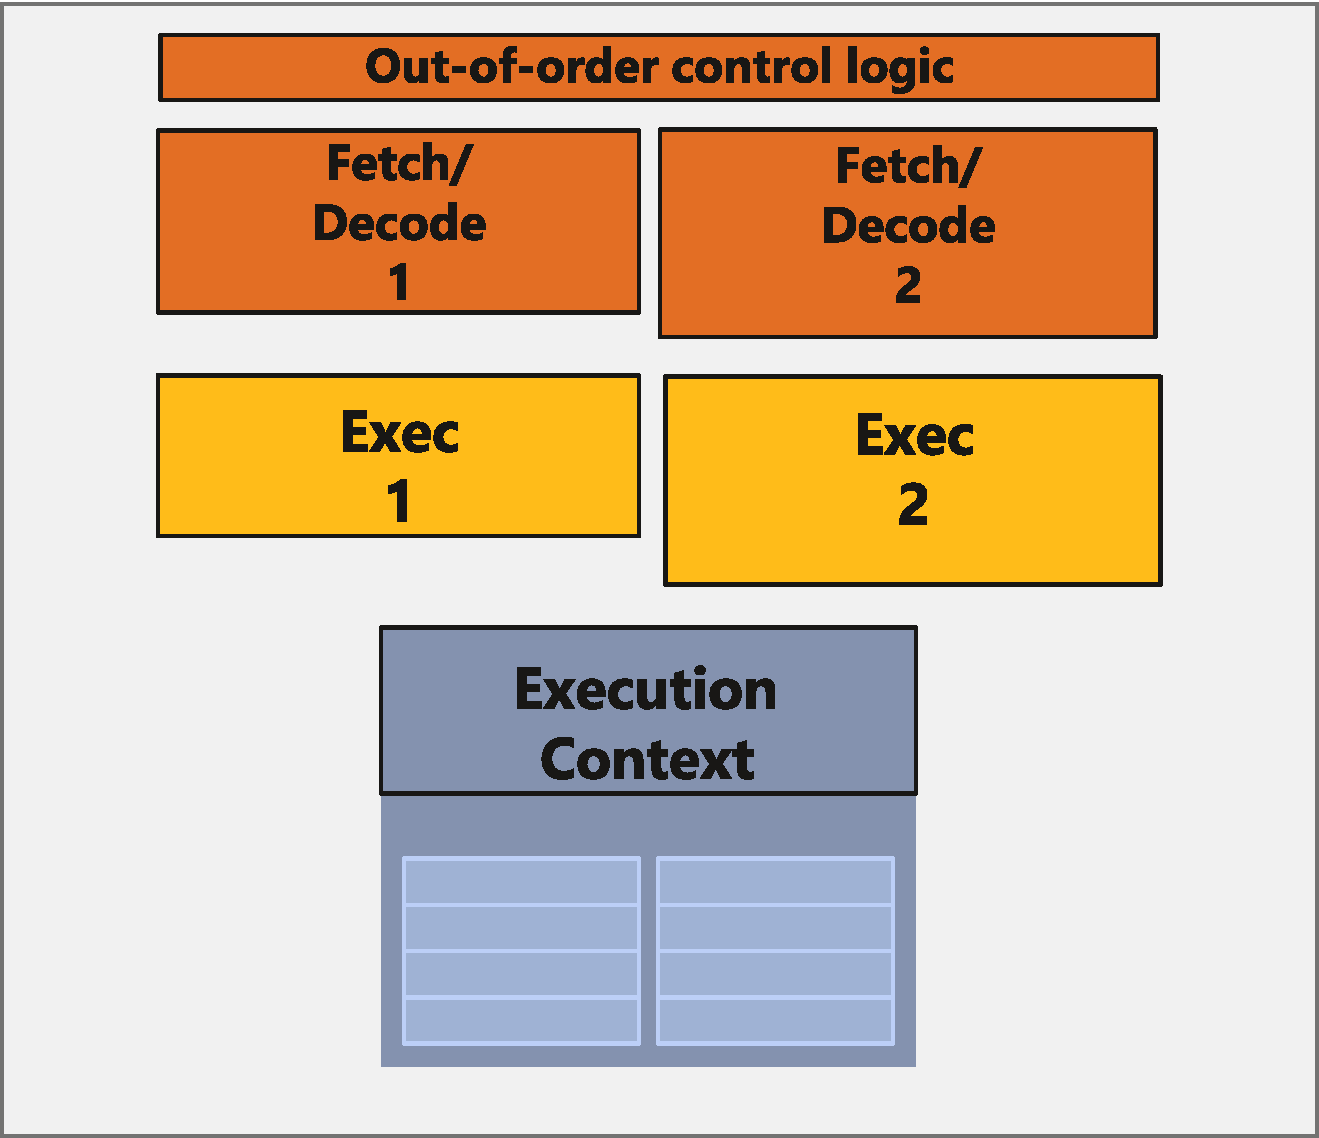
\includegraphics[width=.52\textwidth]{img/superscalar-prcoessor-1.pdf}
    \caption{The superscalar processor.}
\end{figure}

\noindent
The superscalar processor takes advantage of \definition{Instruction-Level Parallelism (ILP)}\footnote{Instruction-level parallelism (ILP) is the parallel or simultaneous execution of a sequence of instructions in a computer program. More specifically ILP refers to the average number of instructions run per step of this parallel execution.} within an instruction stream.
\begin{itemize}
    \item Processing \textbf{different instructions} from the same instruction stream \textbf{in parallel} (\textbf{within a core}).
    \item \textbf{Parallelism is automatically detected by the hardware during execution}.
\end{itemize}

\newpage

\subsubsection{Single Instruction, Multiple Data (SIMD) processor}

Adding execution units (ALUs) to the simplest processor can increase compute capability. Amortize the cost/complexity of managing an instruction stream across many ALUs using \definition{Single Instruction, Multiple Data (SIMD)} processing. Therefore, the \textbf{same instruction is sent to all ALUs}. This \textbf{operation is performed in parallel on all ALUs}.

\begin{flushleft}
    \textcolor{Green3}{\faIcon{check} \textbf{Advantages}}
\end{flushleft}
\begin{itemize}
    \item \textbf{Efficient for data-parallel workloads}: amortize control costs over many ALUs.
    \item Vectorization done by:
    \begin{itemize}
        \item Compiler (\textbf{\underline{explicit SIMD}}): parallelism is explicitly requested by the programmer through intrinsics, conveyed through parallel language semantics, and inferred through loop dependency analysis by the \dquotes{auto-vectorizing} compiler. In other words, the \textbf{SIMD parallelization is done at compile time, and when we inspect the program binary, we can see the SIMD instructions}.

        \item At runtime by hardware (\textbf{\underline{implicit SIMD}}): the \textbf{compiler generates a binary with scalar instructions}, but $n$ instances of the program are always executed together on the processor. The \textbf{hardware} (not the compiler) is \textbf{responsible for the simultaneous execution of the same instruction by multiple program instances on different data on SIMD ALUs}.
    \end{itemize}
\end{itemize}

\longline

\subsubsection{Multi-Core Processor}

A \definition{Multi-Core Processor (MCP)} is a \textbf{microprocessor} on a single integrated circuit (IC) with \textbf{two or more separate central processing units (CPUs)}, called \emph{cores} to emphasize their multiplicity (e.g., \emph{dual-core} or \emph{quad-core}). Each core reads and executes program instructions, specifically ordinary CPU instructions (such as \texttt{add}, \texttt{move data}, and \texttt{branch}). However, the MCP can \textbf{execute instructions on separate cores simultaneously}, \textbf{increasing overall speed for programs that support multithreading or other parallel computing techniques}.
\begin{flushleft}
    \textcolor{Green3}{\faIcon{check} \textbf{Advantages}}
\end{flushleft}
\begin{itemize}
    \item Provides \textbf{thread-level parallelism}: execute a completely different instruction stream on each core simultaneously.
    \item \textbf{Software creates threads to expose parallelism to hardware} (e.g., via threading API)
\end{itemize}
    \subsection{Accessing Memory}\label{subsection: Accessing Memory}

\subsubsection{What is a memory?}

A computer's memory is organized as an array of bytes. Each byte is identified by its address in memory (its position in that array).
\begin{table}[!htp]
    \centering
    \begin{tabular}{@{} c | c @{}}
        \toprule
        Address & Value \\
        \midrule
        \texttt{0x0} & \texttt{16} \\
        \texttt{0x1} & \texttt{255} \\
        \texttt{0x2} & \texttt{14} \\
        \texttt{0x3} & \texttt{0} \\
        \texttt{0x4} & \texttt{0} \\
        \texttt{0x5} & \texttt{0} \\
        \texttt{0x6} & \texttt{6} \\
        \texttt{0x7} & \texttt{0} \\
        \texttt{0x8} & \texttt{32} \\
        \texttt{0x9} & \texttt{48} \\
        \texttt{0xA} & \texttt{255} \\
        \texttt{0xB} & \texttt{255} \\
        \texttt{0xC} & \texttt{255} \\
        \texttt{0xD} & \texttt{0} \\
        \texttt{0xE} & \texttt{0} \\
        \texttt{0xF} & \texttt{0} \\
        \texttt{0x10} & \texttt{128} \\
        \vdots & \vdots \\
        \texttt{0x1F} & \texttt{0} \\
        \bottomrule
    \end{tabular}
    \caption{Example illustration of the program's memory address space of 32 bytes, range from \texttt{0x0} to \texttt{0x1F}.}
\end{table}

\noindent
From the processor's point of view, loading an instruction to access the contents present in memory is done with the \texttt{ld} assembly instruction. For example, \texttt{ld R0 $\leftarrow$ mem[R2]} means \dquotes{take the value from register \texttt{R2} and put that value into register \texttt{R0}}.

\highspace
Before we introduce new concepts, let us take a moment to explain some important \textbf{terminology}:
\begin{itemize}
    \item \definition{Memory Access Latency}, is the \textbf{time} it takes for the \textbf{memory system to deliver data to the processor}.
    
    \item \definition{Processor Stall}. A \textbf{processor} stalls when it \textbf{cannot execute the next instruction in an instruction stream because of a dependency on a previous instruction that has not been completed}. Accessing memory is a major source of stalling, which is one of the main reasons why memory accesses should be limited. 
    \newpage
    For \example{example}, in the following three assembler instructions, the add has to wait for the loading of \texttt{R2} and \texttt{R3} values, making parallelization more complicated:
    \begin{flushleft}
    	\texttt{ld r0 mem[r2]}\newline
    	\texttt{ld r1 mem[r3]}\newline
    	\texttt{add r0, r0, r1}
    \end{flushleft}
    
    \item \definition{Memory Bandwidth}, is the \textbf{rate at which the memory system can provide data to a processor}.

    Bandwidth is the \underline{critical} resource in modern computing.
    
    \textbf{High-performance parallel programs will}:
    \begin{enumerate}
        \item \textbf{Organize computation to fetch data from memory less frequently}. For example, reuse data previously loaded by the same thread (temporal locality optimizations) or share data across threads (inter-thread cooperation);
        
        \item Prefer to \textbf{perform additional arithmetic to store/reload values};
        
        \item \textbf{Programs need to access memory infrequently} to take advantage of modern processors.
    \end{enumerate}
\end{itemize}

\newpage

\subsubsection{How to reduce processor stalls}

\paragraph{Cache}

One of the most common solutions is caching.

\highspace
A \definitionWithSpecificIndex{cache}{Cache}{} is a hardware or software \textbf{component that stores data so that future requests for that data can be served faster}; the data stored in a cache might be the result of an earlier computation or a copy of data stored elsewhere.
\begin{itemize}
    \item A \definition{Cache Hit} occurs when the \textbf{requested data is found} in a cache;
    \item A \definition{Cache Miss} occurs when \textbf{it cannot}.
\end{itemize}
Cache hits are served by reading data from the cache, which is faster than recomputing a result or reading from a slower data store, so the \textbf{more requests that can be served from the cache, the faster the system performs}.\cite{wikipediaCacheResearch}

\highspace
Many modern CPUs have logic that predicts what data will be accessed in the future and \dquotes{pre-fetches} that data into caches. \definition{Prefetching} reduces stalls because the data is resident in the cache when it is accessed. But beware, the other side of the coin is that if the \textbf{guess is wrong}, the \textbf{performance is worse than the system without prefetching}!

\longline

\paragraph{Multi-threading}

A \definition{Multithreaded Processor} is one that has the \textbf{ability to follow multiple instruction streams without software intervention}. In practice, then, this \textbf{includes any machine that stores multiple program counters (PCs) in hardware within the processor} (i.e., on chip, for microprocessor-era machines).\cite{nemirovsky2022multithreading}

\highspace
The main idea in this architecture is to \textbf{interleave processing of multiple threads on the same core to hide stalls}. In other words, if we can't make progress on the current thread, we work on another one.

\begin{examplebox}[: core utilization]\label{example: core utilization}
    To better understand our explanation, suppose we are running a program where threads perform \textbf{three arithmetic instructions followed by a memory load} (with 12 cycle latency).
    \begin{center}
        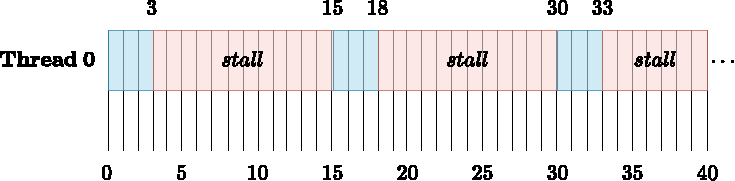
\includegraphics[width=\textwidth]{img/multi-threading-1.pdf}
    \end{center}

    From the figure, it is clear that if we consider an arithmetic instruction and a memory stall, the core is not fully optimized to work at 100\%. In practice, we see that a single arithmetic instruction takes 3 clock cycles and the memory stall takes 12 clock cycles. This means that from this situation we are using the CPU at only 20\% (3 work clock cycles on 15)!

    Without suggesting the final solution, try to see what happens when we add another thread.
    \begin{center}
        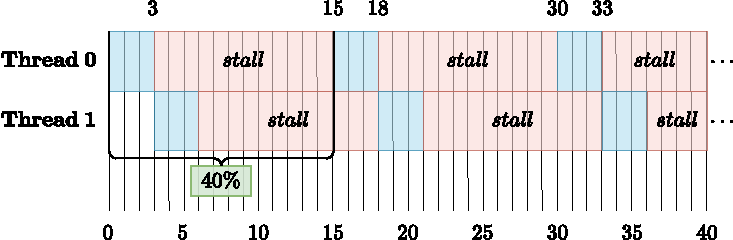
\includegraphics[width=\textwidth]{img/multi-threading-2.pdf}
    \end{center}
    
    We have gained three clock cycles, and now we are taking advantage of the 40\% of the core.

    Now, how many threads do we need to achieve 100\% utilization? The answer is simple: the number of clock cycles of the operations to be done before the stall plus the clock cycles of the stall divided by the working operations (operations that are not stalls). In our case: $15 \div 3 = 5$.
    \begin{center}
        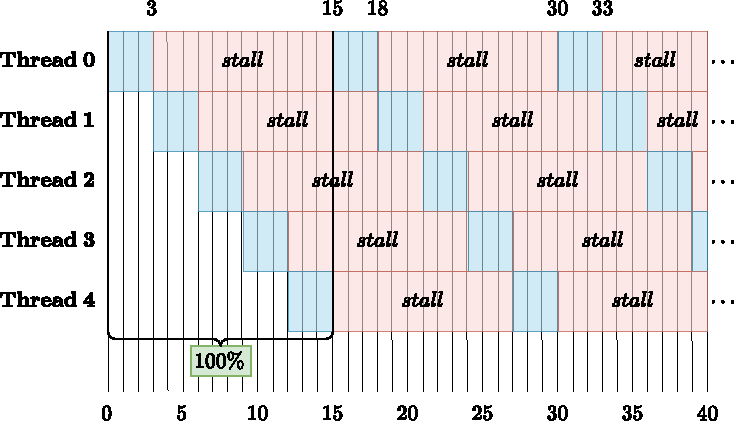
\includegraphics[width=\textwidth]{img/multi-threading-3.pdf}
    \end{center}

    Note that if we add more threads, there will be no benefit because the CPU is already at 100\%.
\end{examplebox}

\begin{flushleft}
    \textcolor{Green3}{\faIcon{check} \textbf{Multithreaded Processor benefits}}
\end{flushleft}
\begin{itemize}
    \item A processor with multiple hardware threads has the \textbf{ability to avoid stalls} by executing instructions from other threads when one thread must wait for a long latency operation to complete. The latency of the memory operation is not changed by multithreading, it just no longer causes reduced processor utilization.
    
    \item A \textbf{multithreaded processor hides memory latency by performing arithmetic from other threads}. Program that feature more arithmetic per memory access need fewer threads to hide memory stalls.
\end{itemize}

\begin{flushleft}
    \textcolor{Red2}{\faIcon{microchip} \textbf{Type of hardware-supported multithreading}}
\end{flushleft}
\begin{itemize}
    \item \textbf{Core manages execution contexts for multiple threads}. This type still has the same number of ALU resources: multi-threading only helps to use them more efficiently in the face of high latency operations such as memory access. The \textbf{processor decides which thread to run each clock cycle}.
    
    \item \definition{Coarse-Grain Multithreading}, also called \blackdefinition{Block Multithreading} or \blackdefinition{Switch-On-Event Multithreading}, has multiple hardware contexts associated  with each processor core. A hardware context is the program counter, register file, and other data required to enabled a software thread to execute on a core. However, only one hardware context has access to the pipeline at a time.\cite{nemirovsky2022multithreading}

    \item \definition{Fine-Grain Multithreading (FGMT)}, also known as \blackdefinition{Interleaved Multithreading} or \blackdefinition{Temporal Multithreading}, is the type just described on the previous pages, as in the example on page \pageref{example: core utilization}.

    \item \definition{Simultaneous Multithreading (SMT)} has multiple hardware contexts associated with each core. In a simultaneous multithreaded processor, instructions from multiple threads are available to be issued on any cycle. Therefore, all hardware contexts, and in particular all register files, must be accessible to the pipeline and its execution resources.\cite{nemirovsky2022multithreading}
    
    In other words, \textbf{each clock}, the \textbf{core selects instructions from multiple threads to execute on ALUs}.
\end{itemize}

    %%%%%%%%%%%%%%%%%%%%%%
    % Programming models %
    %%%%%%%%%%%%%%%%%%%%%%
    \section{Programming models}

\subsection{Implicit SPMD Program Compiler (ISPC)}

Before introducing the ISPC compiler, we give the definition of SPMD.

\begin{definitionbox}[: Single Program, Multiple Data (SPMD)]
    \definition{Single Program, Multiple Data (SPMD)} is a term that has been used to refer to computational models for exploiting parallelism, where \textbf{multiple processors work together to execute a program to achieve faster results}.

    The \textbf{difference} between \emph{SPMD} and \emph{SIMD} (page \pageref{subsubsection: Single Instruction, Multiple Data (SIMD) processor}) is that in SPMD parallel execution, \textbf{multiple autonomous processors simultaneously execute the same program at independent points}, rather than in SIMD it is vectorization at the instruction level so that \textbf{each CPU instruction processes multiple data elements}.

    In other words:
    \begin{itemize}
        \item SPMD: is the \textbf{programming abstraction}, because the programmer has to think; the program is written in terms of this abstraction.
        \item SIMD: in general, the compilers (ISPC) issue special vector instructions that execute the logic performed by each parallel instance created (ISPC gang spawned). In addition, the compilers handle the mapping of conditional control flow to vector instructions.
    \end{itemize}
    The difference and the terminology used by ISPC will become clearer in the following pages. We suggest that finish this section and come back here in a moment.
\end{definitionbox}

\begin{definitionbox}[: Implicit SPMD Program Compiler (ISPC)]
    \definition{Implicit SPMD Program Compiler (ISPC)} is a \textbf{compiler for a variant of the C programming language}, with extensions for \emph{Single Program, Multiple Data (SPMD)} programming. Under the SPMD model, the programmer writes a program that generally appears to be a regular serial program, though the execution model is actually that a number of program instances execute in parallel on the hardware. In other words, the \textbf{ISPC gives the programmer some API to do parallelization on the code; it also generates high quality SIMD code to increase performance}.
\end{definitionbox}

\noindent
The definition, implementation, and other details are explained in the official \href{https://github.com/ispc/ispc}{Intel GitHub repository}.

\newpage

\begin{flushleft}
    \textcolor{Green3}{\faIcon{question-circle} \textbf{How it works?}}
\end{flushleft}
Let us take a general main program; when we call an \texttt{ispc} function, it causes a \textbf{spawn of gang of ISPC program instances upon return, all instances have completed}. These \textbf{instances execute the same ISPC code simultaneously}, and \textbf{each instance has its own copy of local variables}. Take the following ISPC code as an example:
\begin{lstlisting}[language=c++, mathescape]
export void ispc_sinx(
    uniform int N, $\label{code: uniform}$
    uniform int terms,
    uniform float* x,
    uniform float* result
){
    // assume N % programCount = 0
    for (uniform int i=0; i<N; i+=programCount) { $\label{code: programCount}$
        int idx = i + programIndex; $\label{code: programIndex}$
        float value = x[idx];
        float numer = x[idx] * x[idx] * x[idx];
        uniform int denom = 6; // 3!
        uniform int sign = -1;
        for (uniform int j=1; j<=terms; j++) { 
            value += sign * numer / denom
            numer *= x[idx] * x[idx];
            denom *= (2*j+2) * (2*j+3);
            sign *= -1;
        }
        result[idx] = value;
    }
}
\end{lstlisting}
In the example, the \texttt{programCount} (row \ref{code: programCount}) and \texttt{programIndex} (row \ref{code: programIndex}) variables, \texttt{uniform} (row \ref{code: uniform}, and so on) data type tell us:
\begin{itemize}
    \item \texttt{programIndex} gives the index of the SIMD-lane being used for running each program instance (in other words, it's a varying \textbf{integer value that has value zero for the first program instance, and so forth}).
    
    \item \texttt{programCount} gives the \textbf{total number of instances in the \emph{gang}}.
    
    \item A variable that is declared with the \texttt{uniform} qualifier represents a \textbf{single value that is shared across the entire \emph{gang}}. 
\end{itemize}
Together, these can be used to uniquely map executing program instances to input data (\href{https://ispc.github.io/ispc.html#parallel-iteration-with-programindex-and-programcount}{programIndex and programCount}, \href{https://ispc.github.io/ispc.html#uniform-data}{uniform data type}).

\highspace
With the ISPC analogy, the \definition{SPMD programming model} should be clear:
\begin{enumerate}
    \item \textbf{Single thread of control} (typically a main program);
    \item \textbf{Invoke} the \textbf{SPMD function} (in the previous example, the \texttt{ispc\_sinx} function);
    \item \textbf{SPMD execution}, then \textbf{multiple instances of the function run in parallel} (multiple logical threads of control);
    \item \textbf{Returns} and \textbf{resumes a single thread} of control.
\end{enumerate}

\newpage

\begin{figure}[!htp]
    \centering
    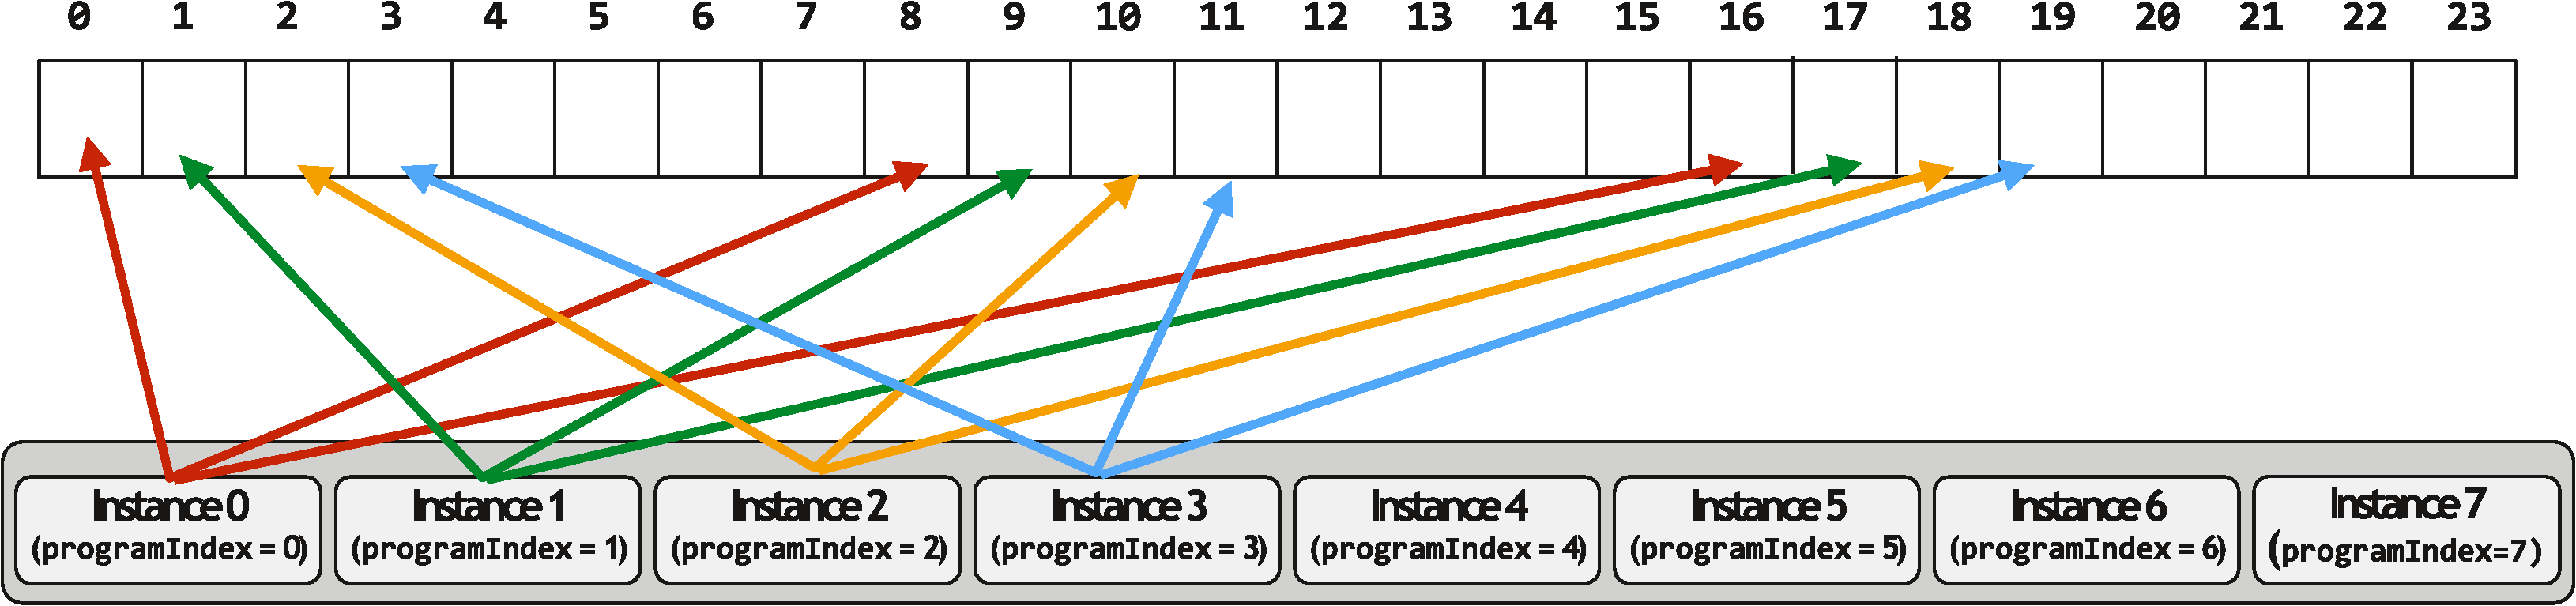
\includegraphics[width=\textwidth]{img/ispc-1.pdf}
    \begin{center}
        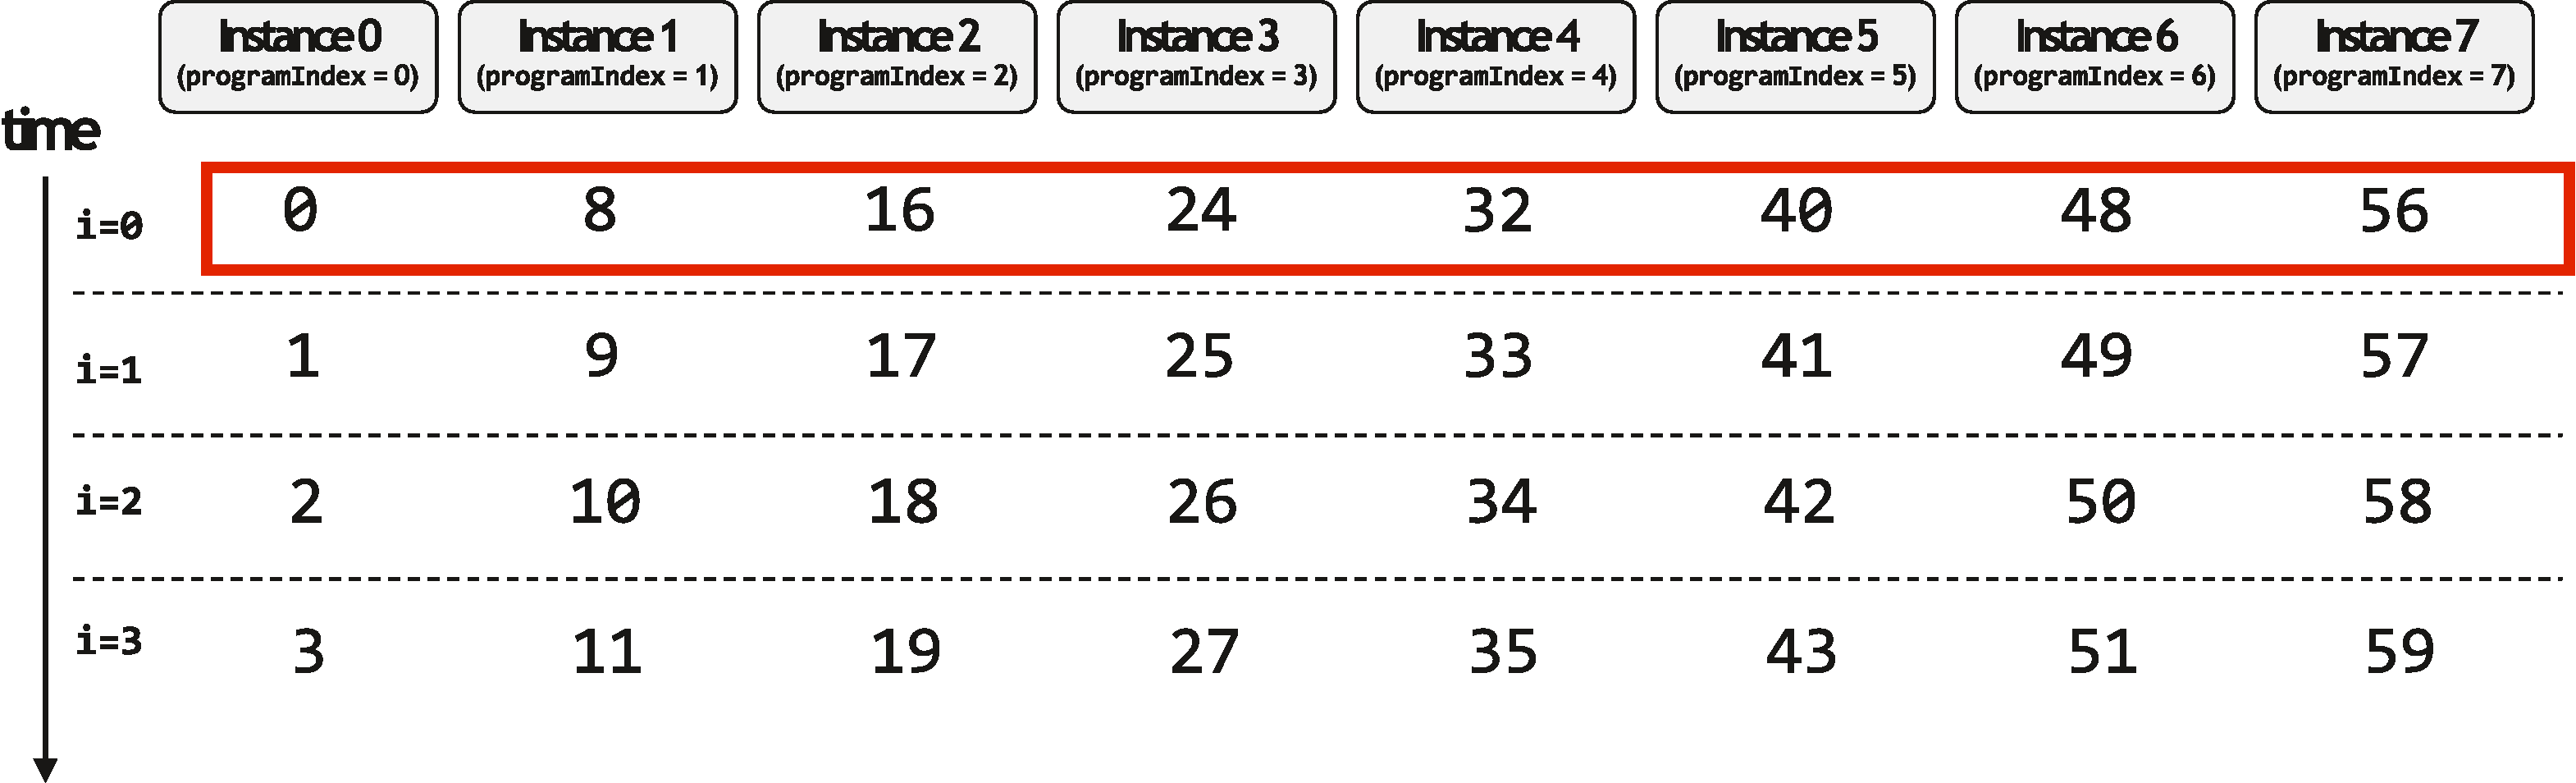
\includegraphics[width=\textwidth]{img/ispc-2.pdf}
    \end{center}
    \caption{Example of execution with 8 instances (\texttt{programCount} equal to 8). For all program instances, there are eight non-contiguous values in memory. A special instruction called \texttt{gather} is needed to implement this, but unfortunately it is a more complex and expensive SIMD instruction rather than a contiguous implementation.}
    \label{fig: ispc 8 instances, no optimized}
\end{figure}

\noindent
Figure \ref{fig: ispc 8 instances, no optimized} shows a possible execution of the ISPC function using 8 instances. The result is obtained and all is well. But there is one interesting observation. \textbf{Each ISPC instance writes each value in a non-contiguous way}. This can be done better:
\begin{lstlisting}[language=c++, mathescape]
export void ispc_sinx_v2(
    uniform int N,
    uniform int terms,
    uniform float* x,
    uniform float* result
){
    // assume N % programCount = 0
    uniform int count = N / programCount;
    int start = programIndex * count;
    for (uniform int i=0; i<count; i++) {
        int idx = start + i;
        float value = x[idx];
        float numer = x[idx] * x[idx] * x[idx];
        uniform int denom = 6; // 3!
        uniform int sign = -1;
        for (uniform int j=1; j<=terms; j++) { 
            value += sign * numer / denom
            numer *= x[idx] * x[idx];
            denom *= (j+3) * (j+4);
            sign *= -1;
        }
        result[idx] = value;
    }
}
\end{lstlisting}
\newpage
\begin{figure}[!htp]
    \centering
    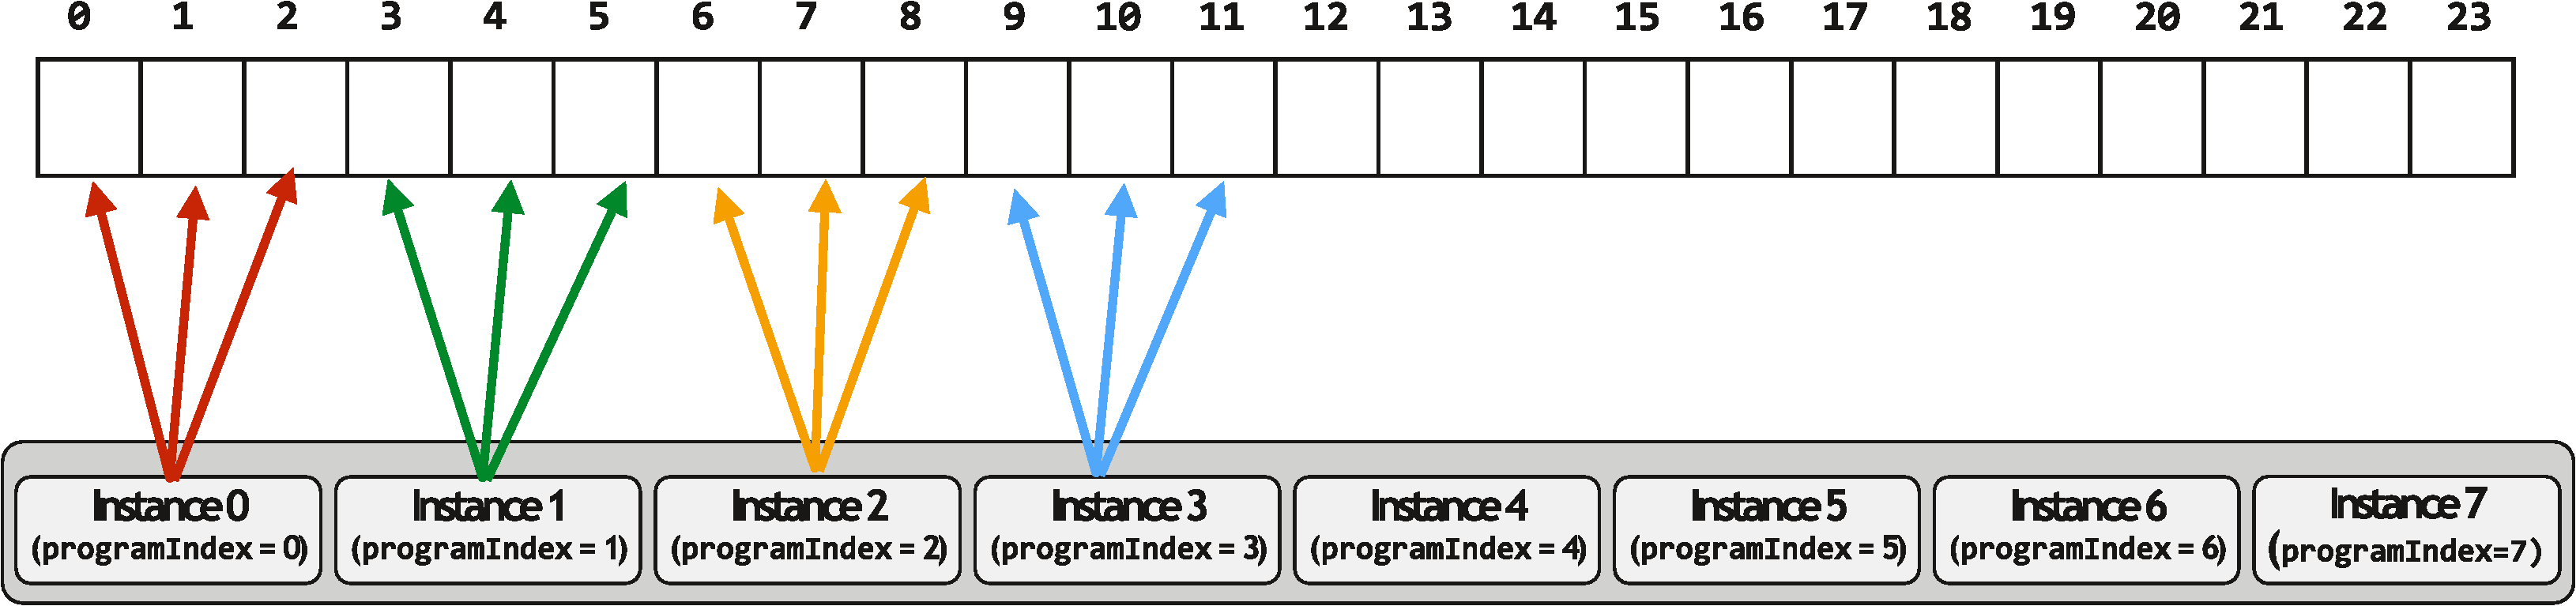
\includegraphics[width=\textwidth]{img/ispc-3.pdf}
    \begin{center}
        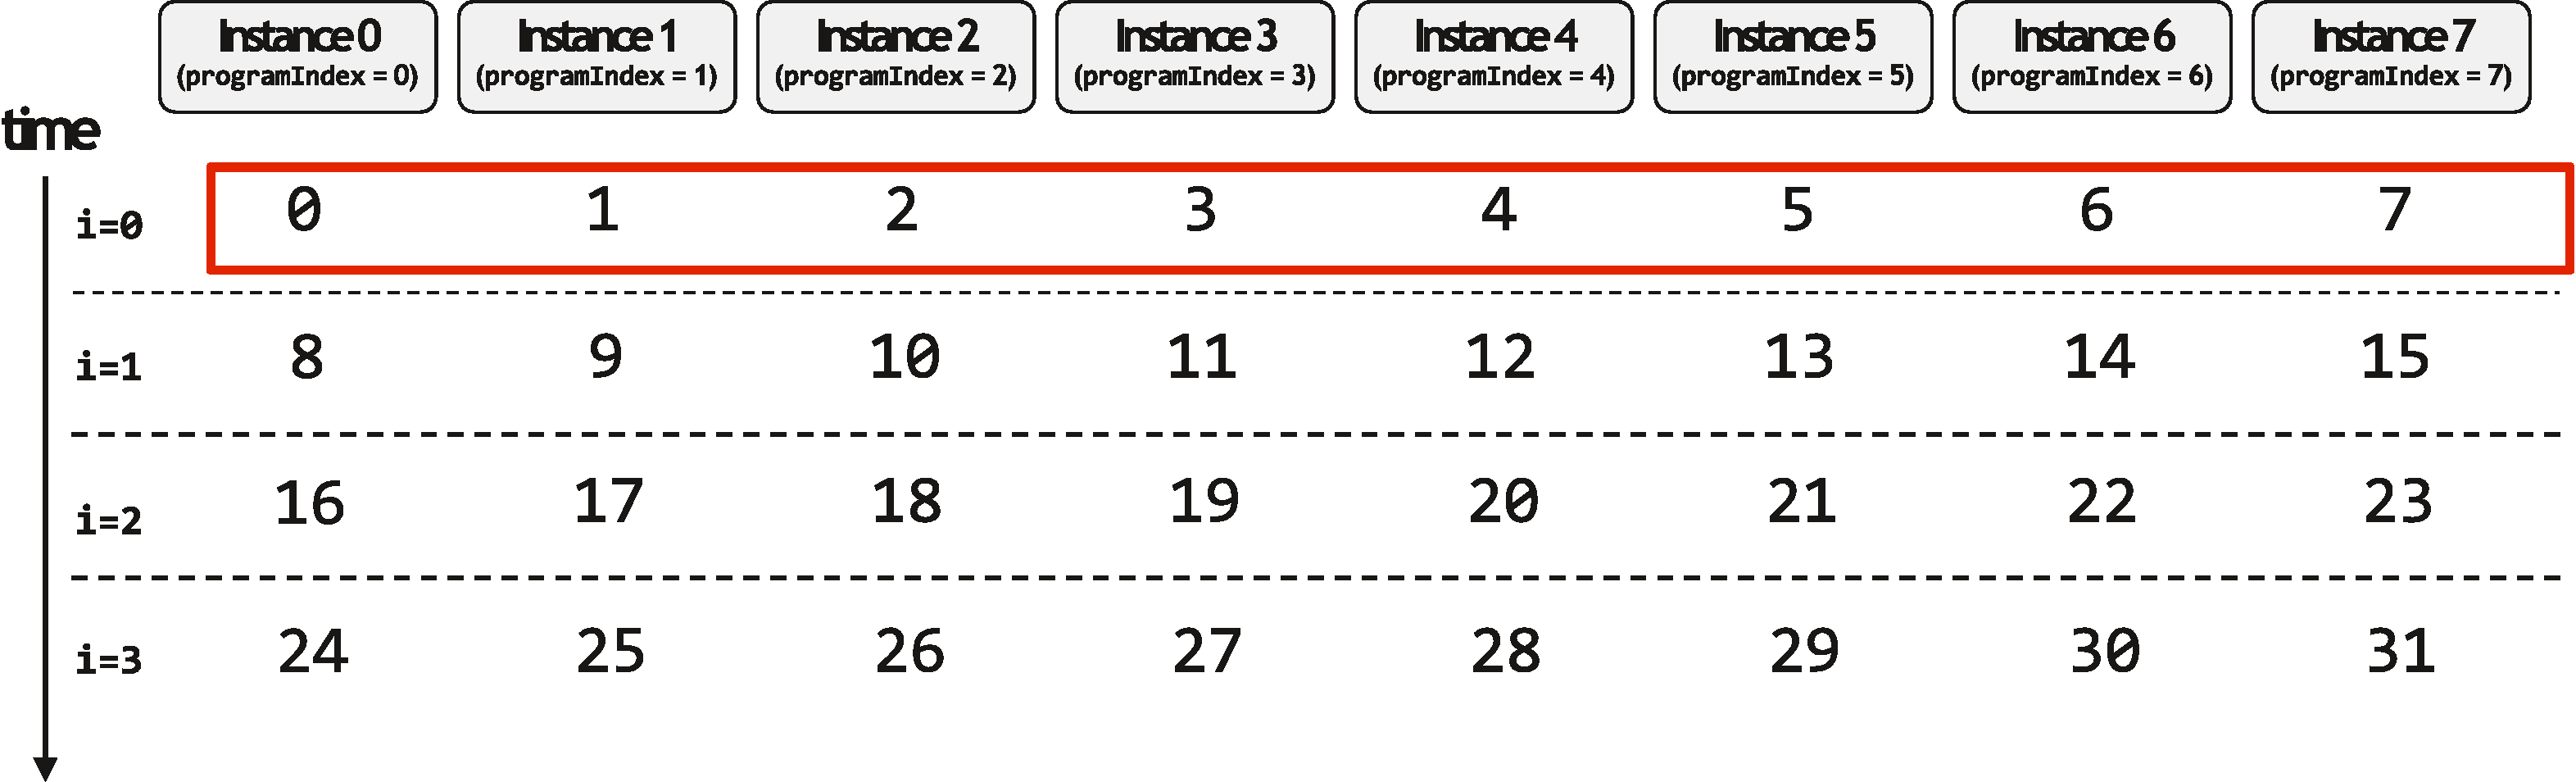
\includegraphics[width=\textwidth]{img/ispc-4.pdf}
    \end{center}
    \caption{Example of execution with 8 instances (\texttt{programCount} equal to 8). A single \dquotes{packed vector load} instruction efficiently implements this. For all program instances, since the eight values are contiguous in memory.}
\end{figure}

    %%%%%%%%%%%%%%%%%%%%%%%%%%
    % Bibliography and index %
    %%%%%%%%%%%%%%%%%%%%%%%%%%
    \pagestyle{fancy}
\fancyhead{} % clear all header fields
\fancyhead[R]{\nouppercase{\leftmark}}

\bibliography{bibtex}{}
\bibliographystyle{plain}

\newpage

\printindex
\end{document}